\section{Distributed Control Flow}
\label{sec:control}

The input to \name is the backend of the Spatial IR, which is an control hierarchy after loop
unrolling.
The controller at each level of the hierarchy corresponds to a control primitive, such as a loop, or
a branch statement. A basic block is attached to each \emph{inner most} controller including instructions
and memory accesses to user declared data-structures.
\Cref{fig:spatialir} shows an example of a program and a schematic Spatial output IR.

\begin{figure*}
\centering
\begin{subfigure}[b]{0.4\textwidth}
\inputminted{python}{code/spatialeg.py}
\caption{Pseudo Spatial Example}
\end{subfigure}
\hfill
\begin{subfigure}[b]{0.58\textwidth}
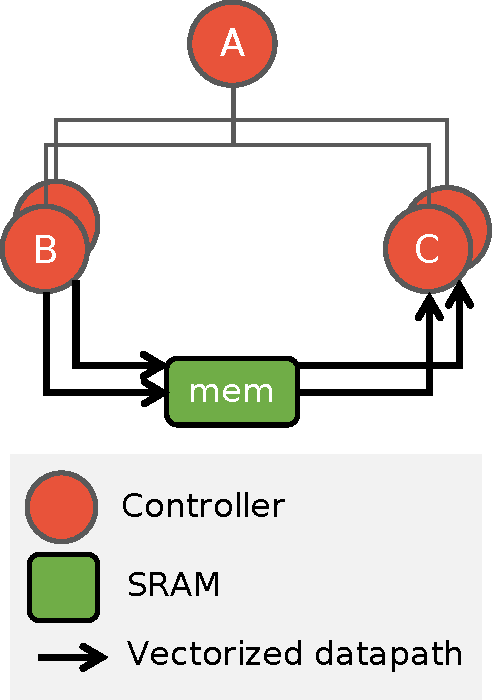
\includegraphics[width=1\textwidth]{figs/spatialir.pdf}
%\missingfigure[figwidth=1\textwidth]{Spatial IR}
\caption{Schematic Spatial IR}
\label{fig:spatialir}
\end{subfigure}
\caption[Spatial Example]{Pseudo example of \name's front-end language}
\end{figure*}

\begin{figure*}
\centering
%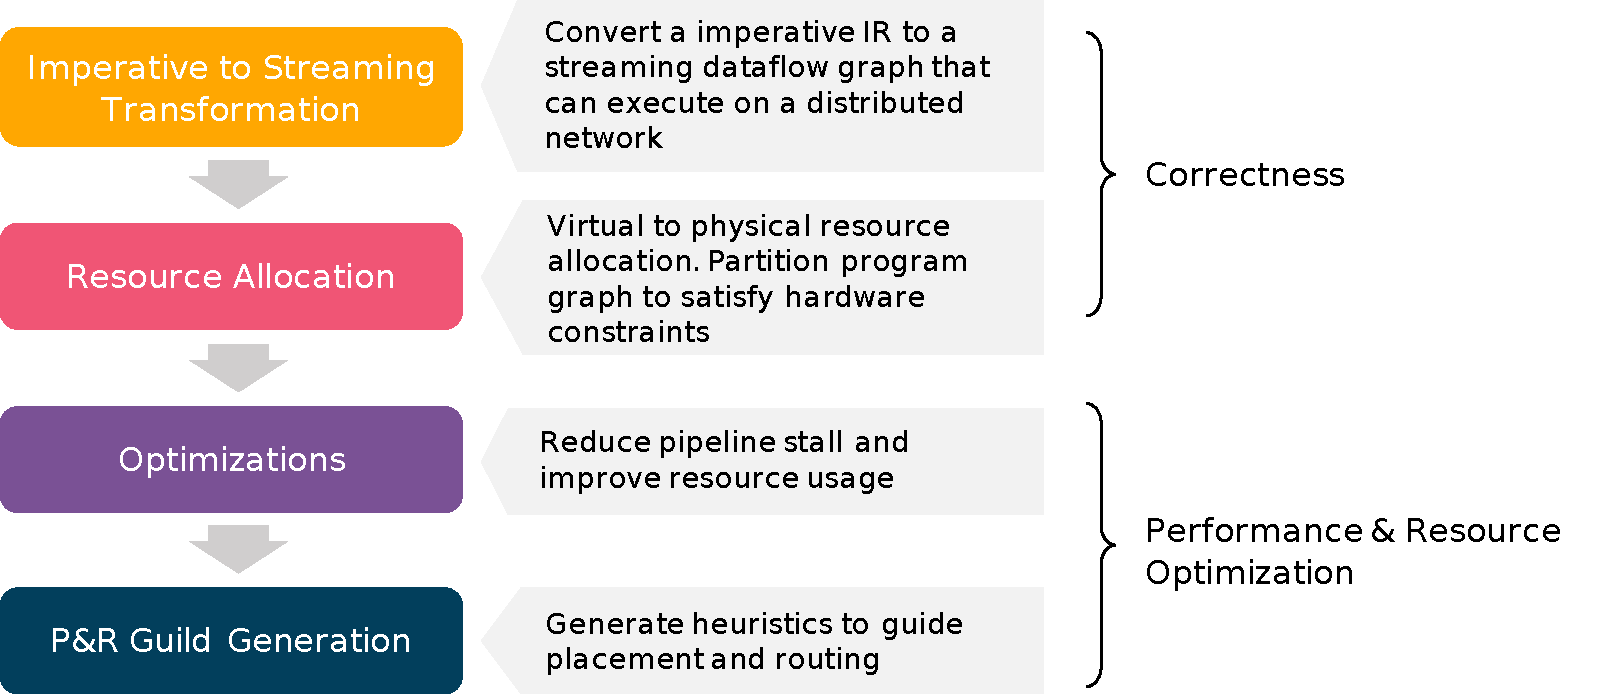
\includegraphics[width=1\textwidth]{figs/sarastack.pdf}
\missingfigure[figwidth=1\textwidth]{Controller duplication}
\caption[Context allocation]{Context allocation}
\label{fig:contextalloc}
\end{figure*}

%\begin{figure*}
%\centering
%\caption[Spatial IR]{Spatial IR}
%\label{fig:spatialir}
%\end{figure*}

As a start, \name allocates one virtual memory to hold each on-chip data structure, and 
one context to execute each basic block within the inner most controllers. 
A basic block maps naturally to a context, as instructions within a basic block are control-free. 
Next, \name makes a copy of all controllers enclosing the basic block in the corresponding context, as
shown in \Cref{fig:contextalloc};
these controllers are later converted to counters and control configurations supported by the
hardware. 
With these controllers, contexts can repeat execution for expected number iterations. However,
data-structures written and read by different contexts are accessed in random order.
The insight is that \emph{as long as all contexts accessing a shared memory with expected program order,
the final result is identical to a sequentially executed program}.
Unlike traditional out-of-order execution, where hardware and compiler look for independent instructions to
execute concurrently, \name starts with all basic blocks executing in concurrent contexts.
\name then introduces synchronizations to maintain consistent access order as expected by the 
program \emph{only} among contexts accessing a shared memory. 
This way, \name introduces minimum p2p synchronizations among small groups of contexts; contexts
accessing different memories are naturally parallelized without impacting the final output.
\todo{walk through an example here}.

To order the execution order or two contexts, \name allocates a single-bit \term{control token} as 
an access grant to the shared memory and passes it between contexts. 
This control token is no different from a regular data-dependency.
By controlling {\em where}, {\em how}, and {\em when} to pass the token, \name 
is able to maintain a consistent update ordering between the pipelined and parallelized actors that access the shared memory.

%In a na\"ive approach, we can map each controller in the hierarchy into a VB (\Cref{fig:centralctrl}).
%This strategy suffers from expensive network round-trip delays between the parent and child controllers.
%If the parent controller is an unrolled loop, the parent needs to synchronize with all child controllers, which creates an undesired communication hot spot.
%\Cref{fig:centralctrl}(a) shows an example where synchronization {\em just} between parent and child controllers can produce an incorrect result due to unpredictable network latency.

%The alternative approach explores a different way to execute the expected control schedule correctly. 
%The minimum required synchronization to produce the correct result is to ensure that the computations access the intermediate results in a consistent matter as if the control schedule is strictly enforced. 
%This can be achieved via p2p synchronizations \emph{only} between computations that access a particular shared memory.
%The execution order of computations that access different memories does not need to be enforced, as they do not impact the program outcome.
%Therefore, as long as the compututation is executed with the expected number of iterations and the memories are updated consistently, there is no need for any extra synchronization.
%Next, we walk through how \name{} achieves this in more concrete detail.


\subsection{Synchronization} 
\label{sec:sync}
We refer to an access to the memory in the input graph as a \emph{declared access}, as supposed to accesses executed at runtime.
For example, multiple accesses across loop iterations are counted as a single declared access.

\paragraph{Where.}
\name only allocate resource to synchronize actors if their declared accesses can potentially interfere.
Whether two declared accesses interfere depends on the type of accesses, the type of the memory, and location of the accesses in the control hierarchy.
For every declared access, \name{} checks other accesses of the same memory appeared earlier in the program order for a possible forward dependency, and later in the program order for a possible loop-carried dependency (LCD). 
Two declared accesses A and B have no dependency if their least-common ancestor (LCA) controller executes only one of the children at anytime (from a branch), or all children in parallel (from an unrolled loop).
The LCD exists between B to A, if B occurs later in the program order, and A and B are surrounded by a loop.
To detect LCD, \name checks if a loop exists among two accesses' LCA controller and LCA's ancestor controllers.
For a dual-ported SRAM, all other accesses need to be synchronized to: share address ports for read-after-read (RAR) and write-after-write (WAW); 
enforce true data-dependency for read-after-write (RAW); and
prevent the overriding of read data for write-after-read (WAR).
\gist{If the memory is multi-buffered (by the user or high-level compiler), we do not need to synchronize for WAR~\cite{dhdl} (the writer writes to a different buffer than the reader does). }
The DRAM interface permits concurrent read streams and, hence, RAR does not need to be synchronized.

\begin{figure*}
\centering
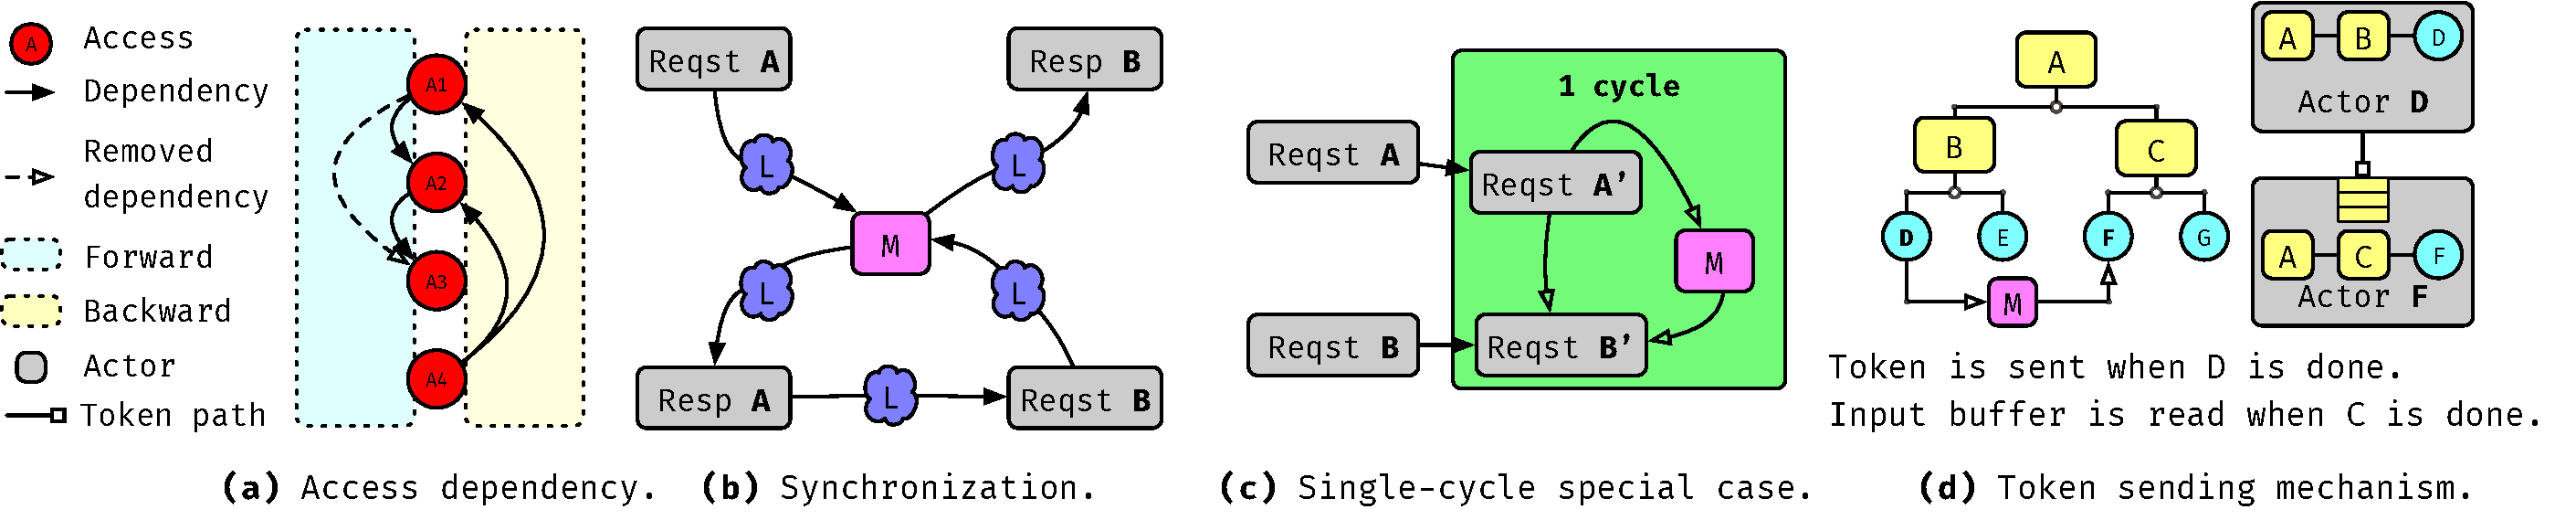
\includegraphics[width=1.0\textwidth]{figs/synch_mech.pdf}
\caption{
    (a) Access dependency graph.
    (b) Synchronization of two accesses on the same memory.
    (c) Single-cycle special case.
    (d) Actors uses local states of controller hierarchy to determine when to send a token.
}\label{fig:depgraph}\label{fig:token}\label{fig:tokentrick}\label{fig:tokenwhen}
\end{figure*}
%\ms{repeated caption, rather give a single caption.}

\paragraph{How.} For each intermediate memory, \name{} builds a dependency graph for all its declared accesses (\Cref{fig:depgraph}(a)).
Enforcing all dependencies in this graph may not be necessary as dependencies between $A_1$ and $A_2$, and $A_2$ and $A_3$ already capture the dependency between $A_1$ and $A_3$.
Therefore, \name{} performs a transitive reduction (TR) on the graph to keep the minimum number of dependency edges that preserve the same ordering \cite{tr}.
Since TR on a cyclic graph is NP-hard, we perform TRs on the forward and backward LCD graphs, separately.
Notice, dependencies between accesses touching different buffers of a multi-buffered memory is less rigid than accesses touching the same buffer.
Therefore, we can only remove an edge if all dependencies on the equivalent path have a stronger or equivalent dependency strength than the strength of the removed edge.

To eliminate the round-trip overhead between the memory and the computation, 
\name{} duplicates the local states and expressions required to generate the requests in a separate actor as the one that handles the responses.
For write accesses, the memory provides an acknowledgment for each request received, used by \name for synchronization.
The request actor generates requests asynchronously as soon as its data-dependencies are cleared, pushing all requests to memory until back-pressured.
To order a declared access A before a declared access B
\name creates a dummy dependency between the actor that accumulates the response of access A ($resp_A$) and the actor that generates requests for access B ($reqst_B$) (\Cref{fig:token}(b)).
To enforce LCD from access B to access A, \name introduces a token from $resp_B$ to $reqst_A$, and initializes the token buffer (input buffer receiving the token) with one element to enable the execution of the first iteration.
If the LCD is on a multi-buffered memory, the LCD token is initialized with the buffer depth number of elements to enable A for multiple iterations before blocked by access B.

These are general schemes we use on any types of memory (including DRAM and on-chip memories) with unpredictable access latency.

\subparagraph{Special Case: Single-Cycle Access}
For a memory with guaranteed {\em single-cycle} access latency, such as registers and statically banked SRAMs that are guaranteed conflict-free, we can simplify the necessary synchronization (\Cref{fig:tokentrick}(c)).
Instead of synchronizing between $resp_A$ and $reqst_B$, we allocate two stateless actors $reqst_A'$ and $reqst_B'$ within {\emph the same} VB as the accessed memory that forwards requests from $reqst_A$ and $reqst_B$, respectively.
Next, we forward the token going from $reqst_A$ to $reqst_B$ to go through $reqst_A'$ to $reqst_B'$ instead, and configure the token buffer in $reqst_B'$ with the depth of one for serialized schedule and depth of M for multi-buffered schedule. 
We no longer need to insert the LCD token, as the stiff back pressure from the token buffer in $reqst_B'$ will enforce the expected behavior.
This optimization only works if the sender and receiver of the token buffer are physically in a single VB where the memory is located.
In this way, when $reqst_B'$ observes $reqst_A'$s token, $reqst_B'$ is guaranteed to observe the memory update from $reqst_A'$ because the memory also has single-cycle access latency.

\subparagraph{Memory Localization}
We perform another specialization on non-indexable memories (registers or FIFOs), whose all accesses have no explicit read enables.
Instead of treating them as shared memories, \name{} duplicates and maps them to local input buffers in all receivers, no longer requiring tokens.
The sender actor pushes to the network when the token is supposed to be sent, and the receiver dequeues one element from the input buffer when the token is supposed to be consumed.
This dramatically reduces the synchronization complexity of non-indexable memory in the common case.

\paragraph{When.}
\name{} configures the actors to generate the token using their local states at runtime.
For FIFOs, the token is generated and consumed every cycle when the producer and receiver actors are active.
For register, SRAM, and DRAM the program order expects that the producer and consumer writes and inspects the memory once per iteration of their LCA controller, respectively.
Since the producer and receiver both have their outer controllers duplicated in their local state, they have independent views for one iteration of the LCA controller, which is when the controller in their ancestors (that is the immediate child of the LCA controller) is completed (\Cref{fig:tokenwhen}(d)).
The {\em done} signals of these controllers are used to produce and consume the token in actors, independently.

\subsection{Data-Dependent Control Flow}
Using the synchronization discussed in \Cref{sec:sync}, we can support control constructs that typically are not supported on most RDAs, such as branch and a while convergence loop.
The controllers in the input graph can also have data dependencies, such as loop ranges. 
The dynamic-loop ranges are handled as data dependencies to actors with \emph{memory localization} described in \Cref{sec:sync}.
The branch condition is also treated as a data-dependent enable signal of controllers under branch clauses.
If the controller is disabled, it is considered {\em done} immediately.
Output tokens depending on the {\em done} signal will be immediately sent out.
For a memory written inside a branch statement and read outside the branch (with a branch miss), the writer actor immediately sends out the token to the receiver
as soon as the branch condition is resolved. 
With a branch hit, the controller waits until its inner controller completes before raising the {\em done} signal.
%This way, the 
A similar scheme is used to implement the while loop, where the while condition is a data-dependency of stop signal of controller X. 
The producer of the while condition also consumes its own output as an LCD. 
The condition is then broadcast to all other actors under the same while loop. 
The {\em done} signal of the while loop is raised when the condition's data-dependency evaluates to true.
At this point, actors accessing memory within the while loop will send the token to access actors outside of the while loop, and enable them to access the intermediate memory.

After all actors and shared resources are allocated and synchronized, we simply put each actor and shared resource into their own VBs.
The actors with single-cycle special case (\Cref{sec:sync}) must be put in the same VB as the shared memory.

